\section{Monte Carlo Corrections}
\label{sec:montecarlocorrections}
The largest corrections to the Monte Carlo arise from inaccurate simulation of lepton selection and trigger efficiencies.
These efficiencies are measured in both the data and simulation, the simulation is then corrected to match the efficiency in the data whenever comparisons are made.
The efficiencies are measured through the use of the Tag \& Probe methodology\cite{TAGANDPROBE}.
In addition to corrections associated with the efficiency of selecting leptons, an additional event scale factor must be applied to account for differences in the pile-up interaction multiplicity between simulation and the data.

\subsection{Trigger Corrections}
\label{subsec:triggercorrections}
The trigger efficiency for the muon leg of a given trigger is measured by first assigning a tag muon that passes the isolated single muon trigger. 
Both the tag and probe muons are required to pass the full identification and isolation requirements outlined in Section \ref{sec:muonselection}.
Finally selected tag and probe muon pairs are only considered if the invariant mass of the di-muon pair lies within a window around the $Z$ mass ($60 < m_{\mu\mu} < 120$ GeV) and the muons have opposite sign.
An efficiency is measured as a function of $p_{T}$ of the probe muon by matching the probe muon to an isolated single muon trigger object.
A functional form of the trigger efficiency is determined by fitting an error function to the measured trigger efficiencies binned in $p_{T}$.
The derived functional form is the ``trigger turn on curve'' shown in the left hand portion of Figure \ref{fig:turnoncurve} with the barrel region on the top and the endcap region on the bottom.
\begin{figure}[ht]
\centering
\begin{minipage}[b]{0.45\linewidth}
\centering
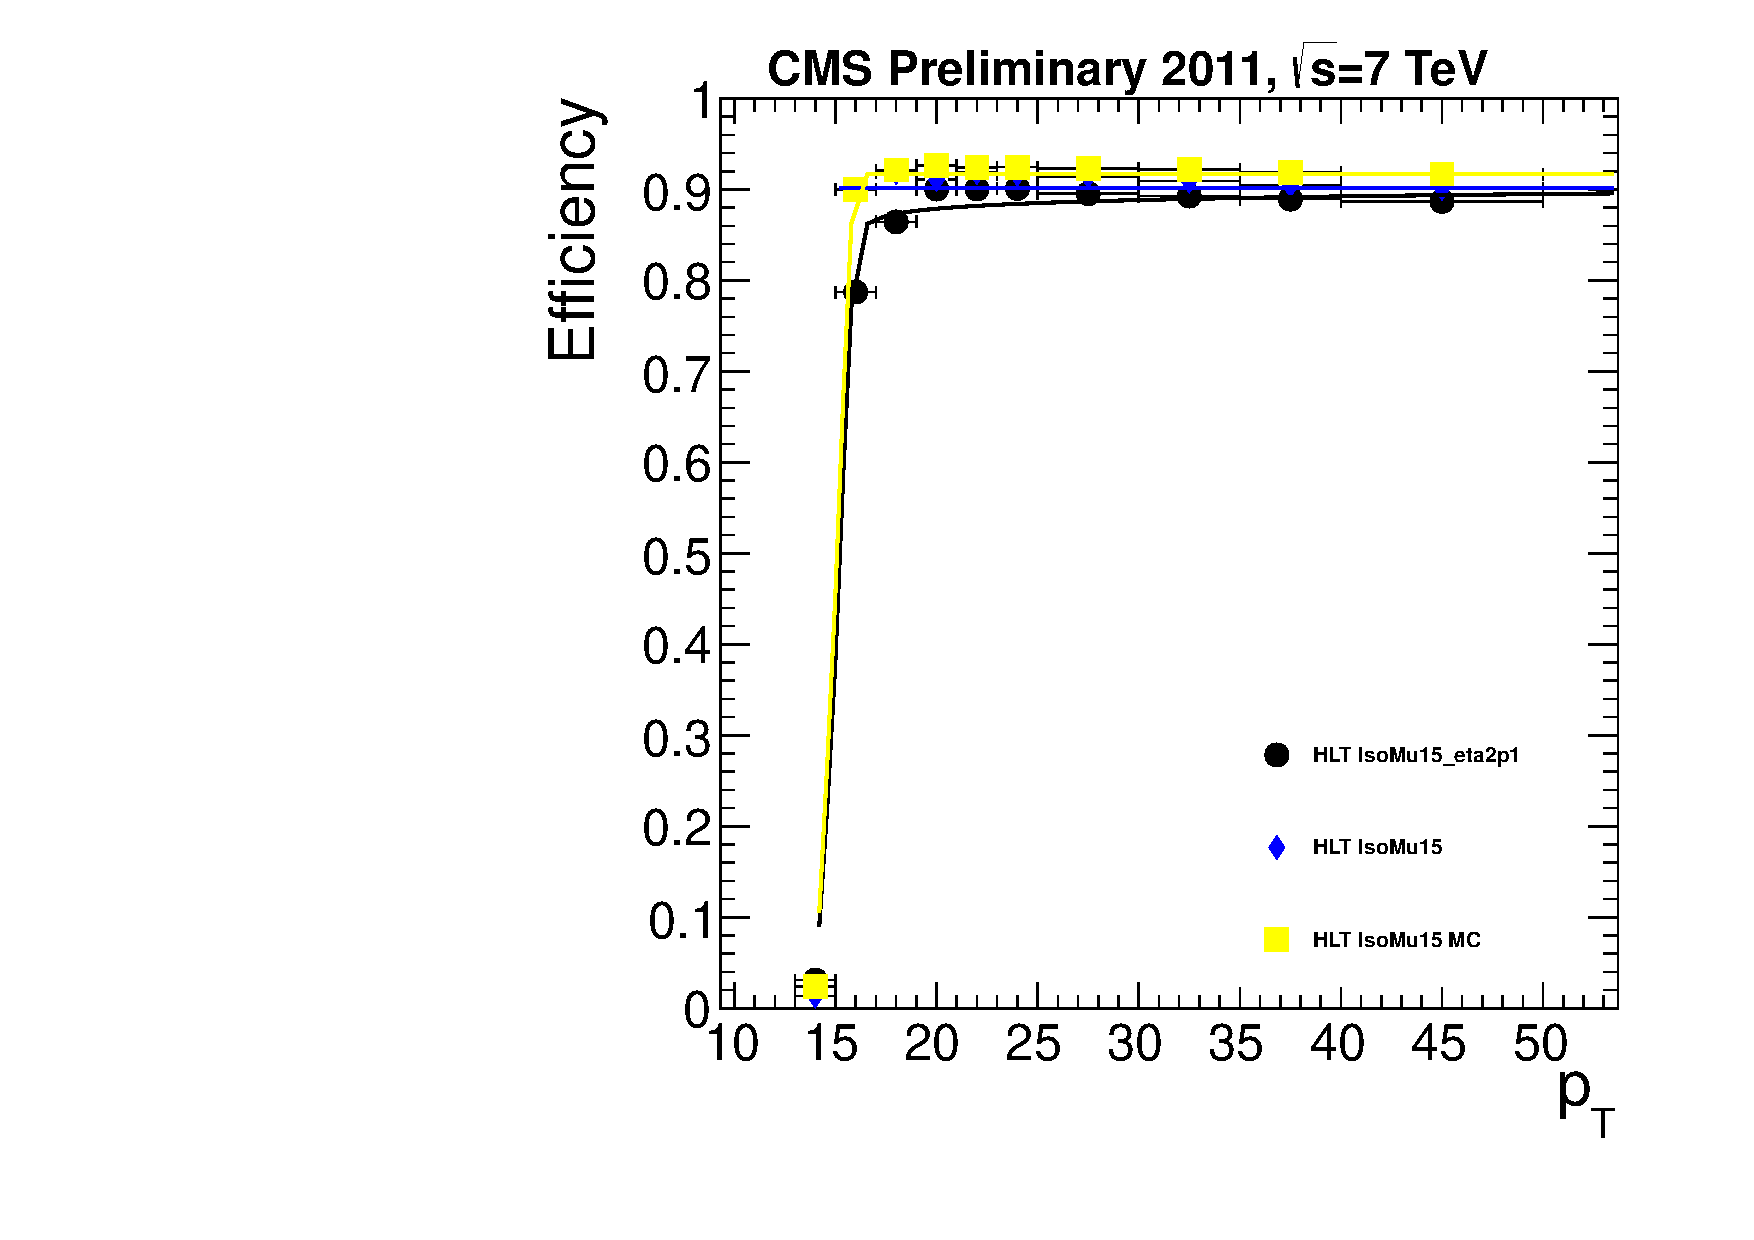
\includegraphics[width=0.9\textwidth]{plots/MuonLegEffB.pdf}
\end{minipage}
\begin{minipage}[b]{0.45\linewidth}
\centering
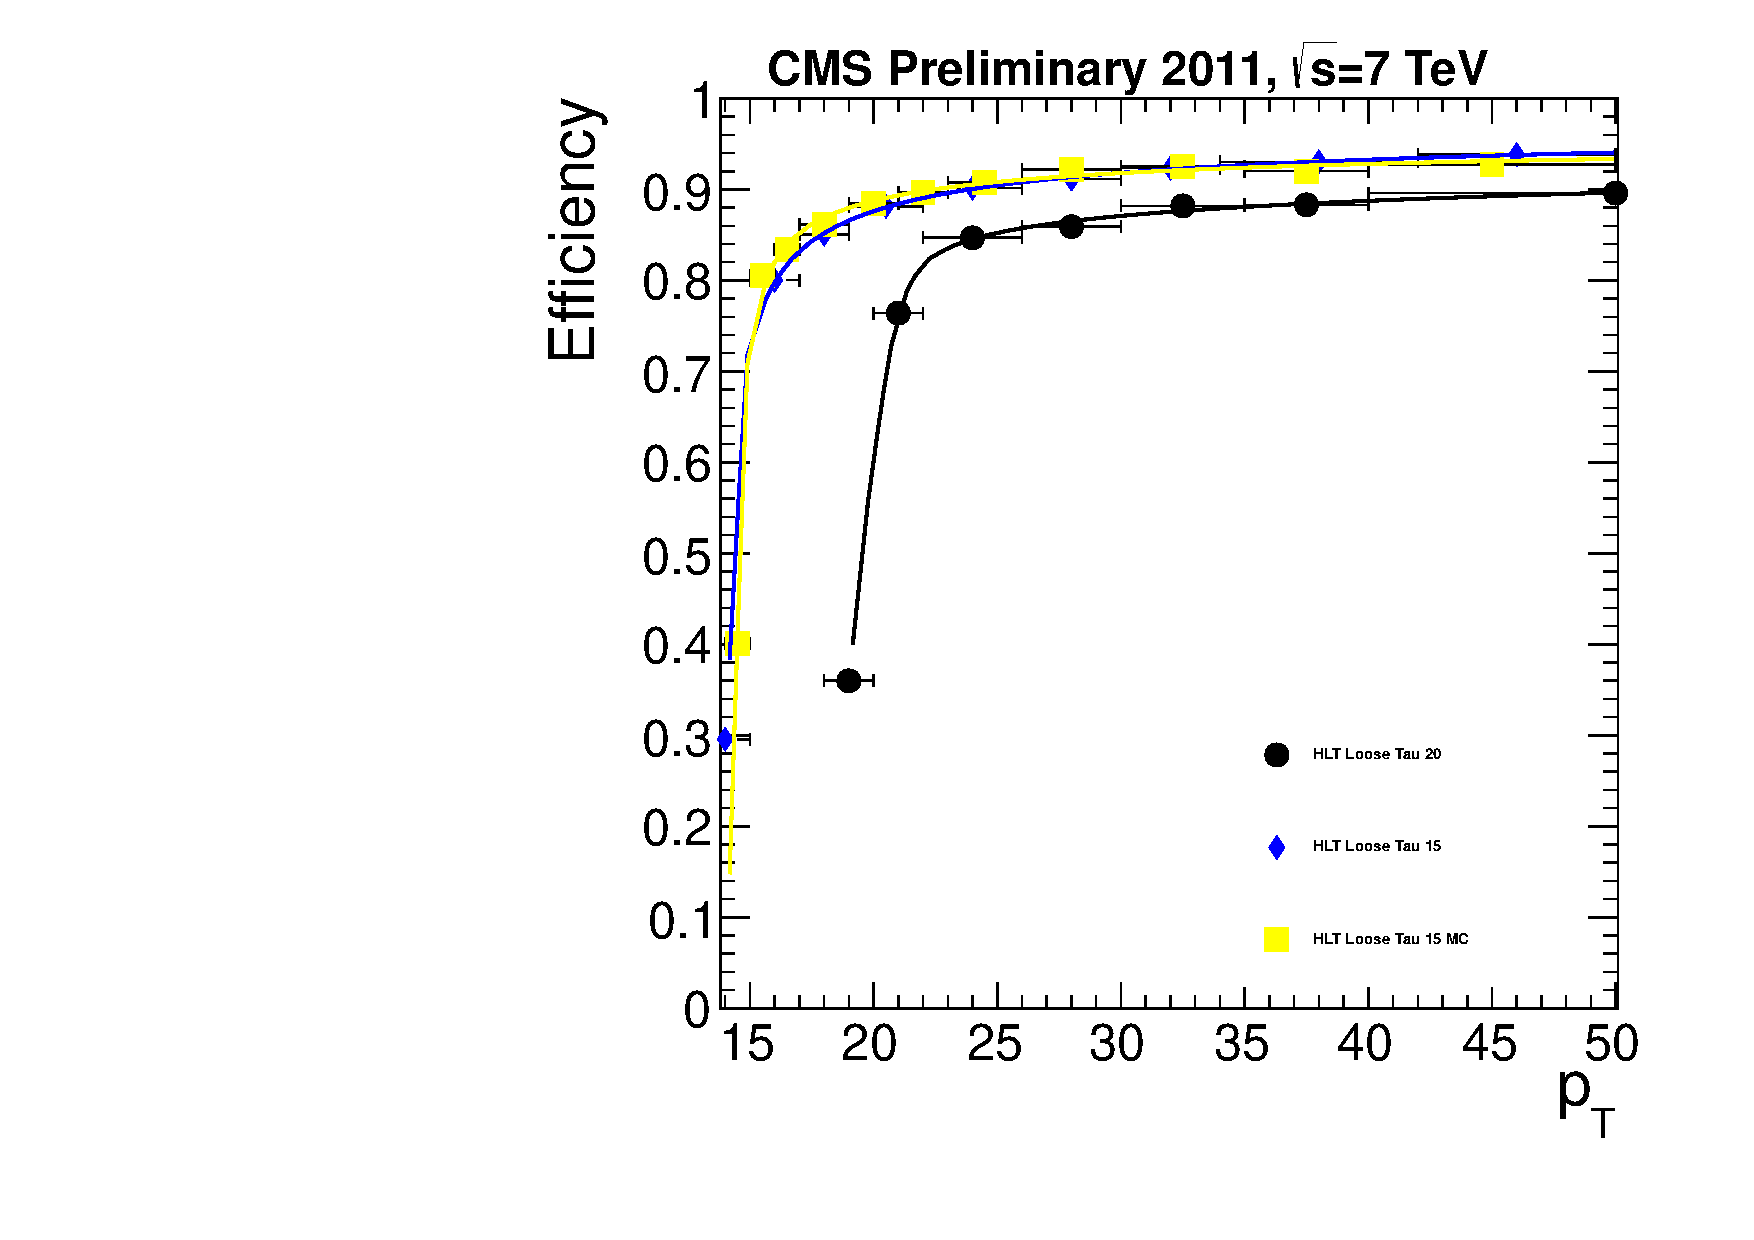
\includegraphics[width=0.9\textwidth]{plots/TauLegEffMuTauB.pdf}
\end{minipage}

\begin{minipage}[b]{0.45\linewidth}
\centering
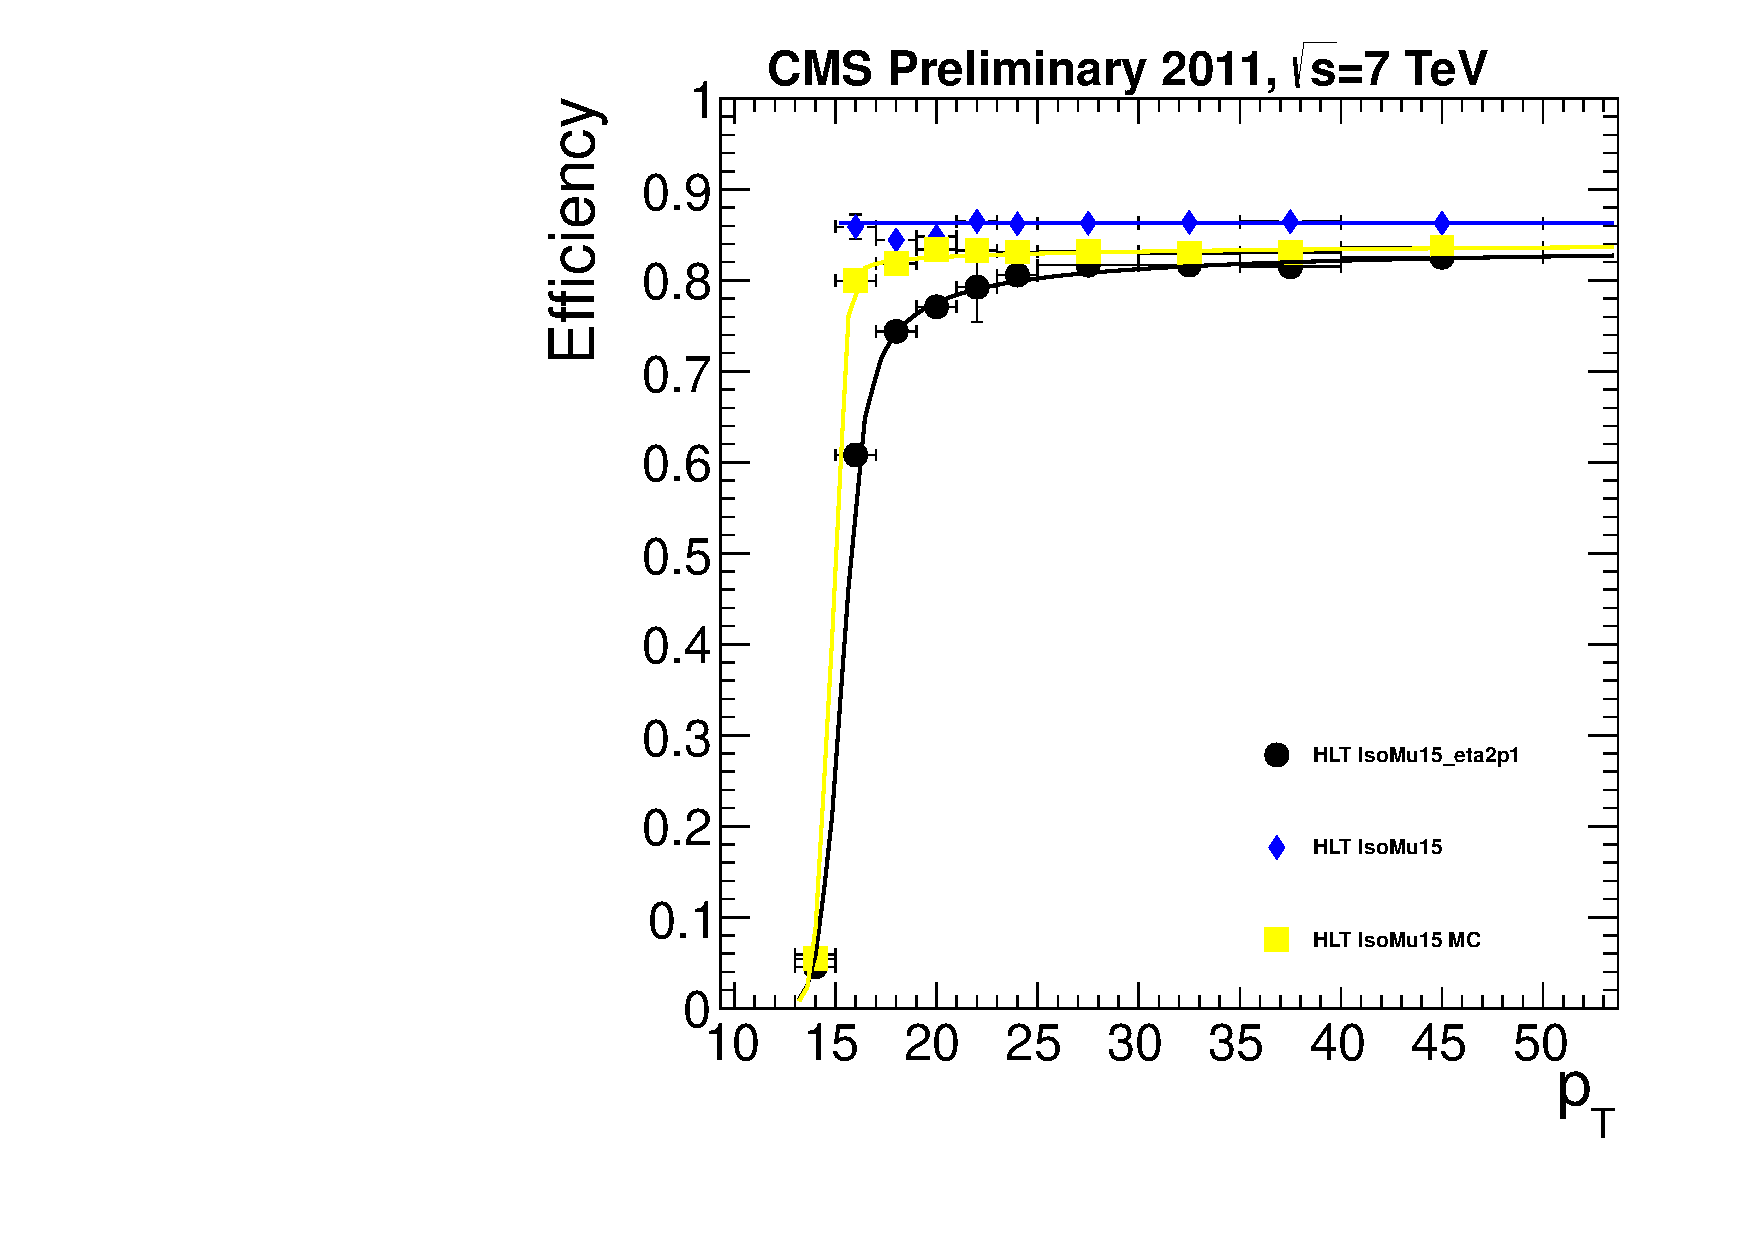
\includegraphics[width=0.9\textwidth]{plots/MuonLegEffE.pdf}
\end{minipage}
\begin{minipage}[b]{0.45\linewidth}
\centering
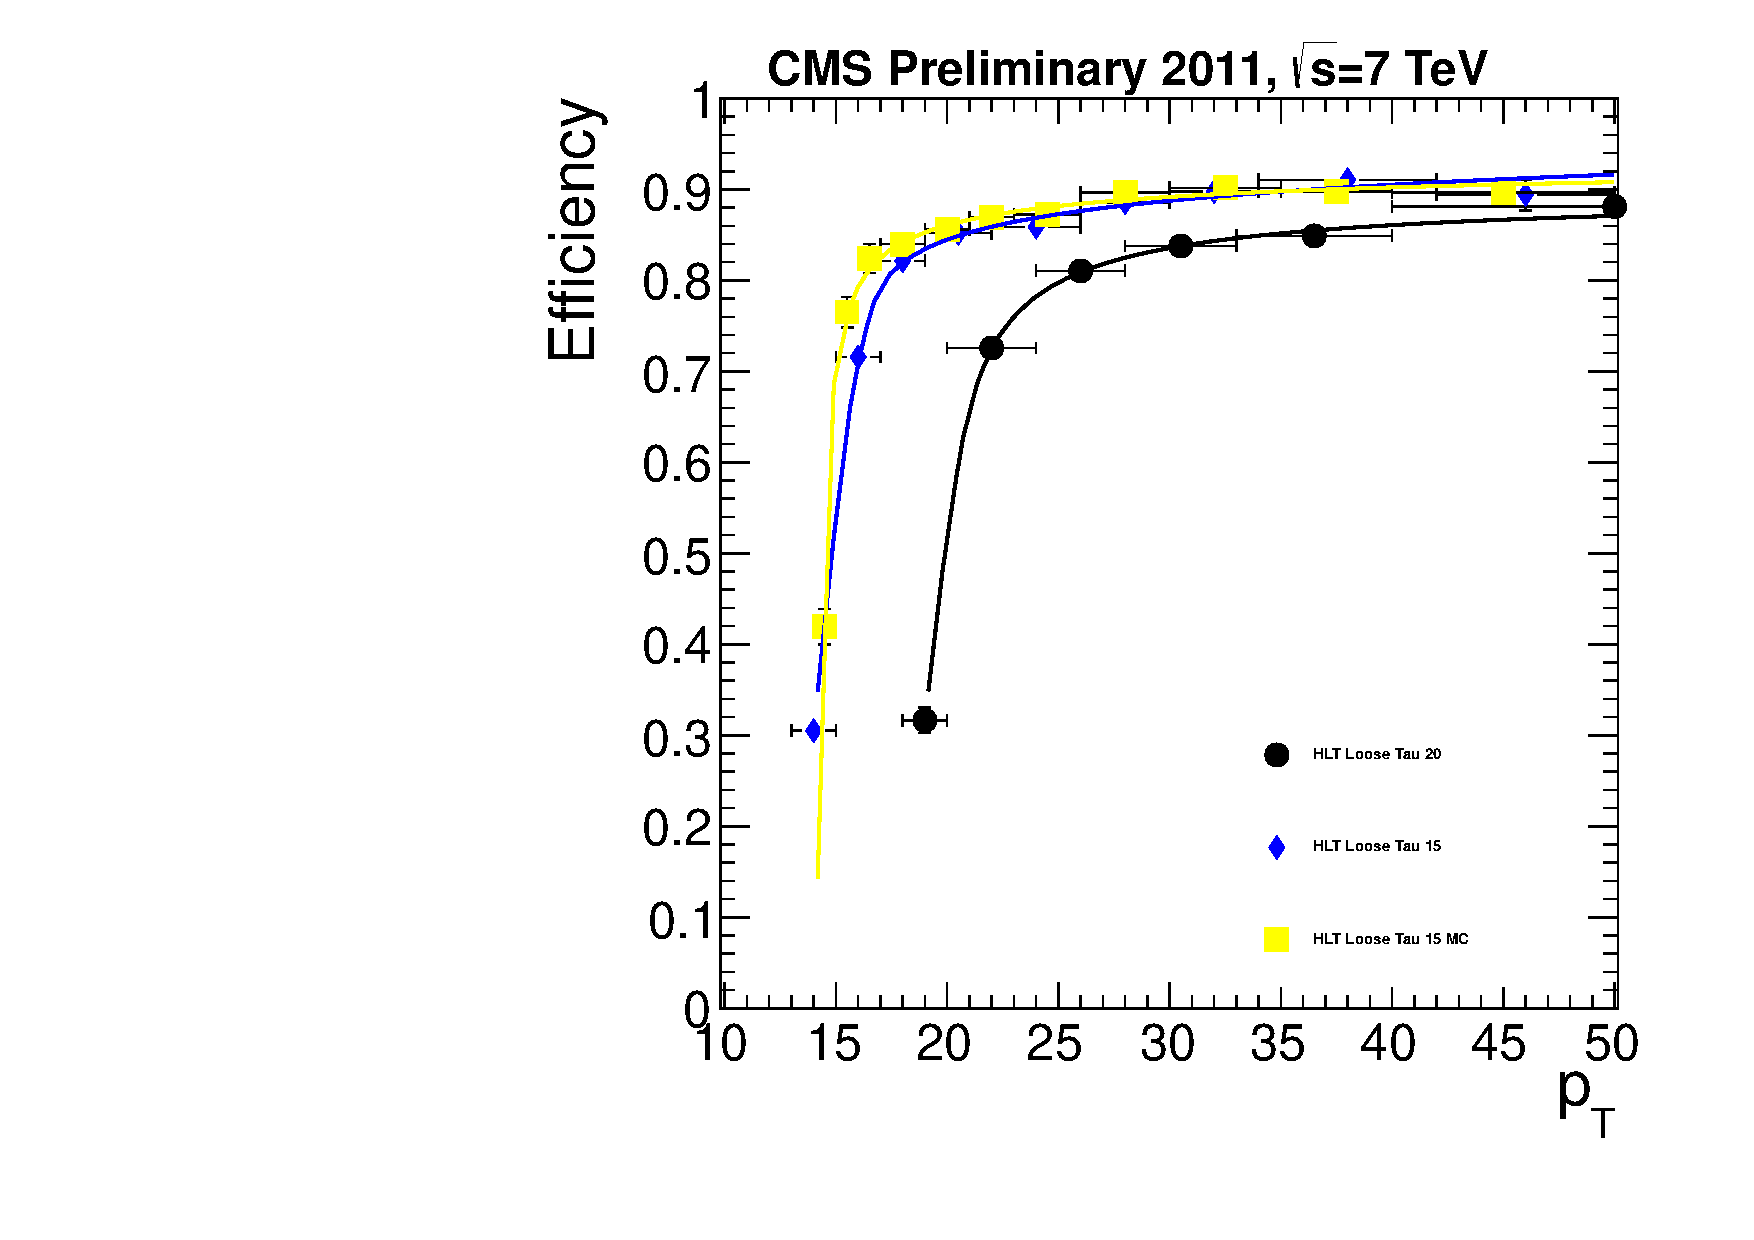
\includegraphics[width=0.9\textwidth]{plots/TauLegEffMuTauE.pdf}
\end{minipage}
\caption{Trigger effeciencies as a function of muon (left) and tau (right) momentum for the barrel (top) and endcap (bottom) regions of the detector.}
\label{fig:turnoncurve}
\end{figure}

A similar procedure is followed to map the efficiency of the tau leg, first selecting a muon that passes the single muon trigger. 
However rather than choosing a probe muon, a probe tau is chosen by making a more loosely selected tau than that described in Section \ref{sec:tauselection}.
The efficiency is again found by fitting an error function to the measured efficiency as a function of the offline reconstructed tau $p_{T}$ and can be seen in the right hand portion of Figure \ref{fig:turnoncurve}, again with the barrel region on top and the endcap region below.

The simulation is then corrected by taking the ratio of the efficiency as measured in simulation to the efficiency as measured in the data.
The final correction is taken as a sum weighted by the luminosity of each trigger used in the data as seen in Table \ref{tab:triggerpaths}.

\subsection{Lepton Selection Corrections}
\label{subsec:leptoncorrections}
The selection efficiencies for muons are calculated with the use of $Z\rightarrow \mu\mu$ events.
A tag and probe method is used in which a tag muon is required to pass all selections listed in Section \ref{sec:muonselection} and match a single muon trigger level object.
The probe muon is then required to satisfy both $p_{T} > 5$ GeV  and $-2.1 < \eta < 2.1$.
The tag and probe muon pairs are then considered if they have opposite charge and an invariant mass within a window around the $Z$ mass: $60 < m_{\mu\mu} < 120$ GeV.
Once tag/probe pairs have been selected, the probe muon is tested to pass the full selection ($N_{pass}$ or $N_{fail}$).
The efficiency is calculated in bins of $p_{T}$, as 
\begin{equation}
\epsilon = {N_{pass}\over N_{pass} + N_{fail}},
\end{equation}
and are summarized in Table \ref{tab:corrections}

\begin{table}[htpb]
\begin{center}
\caption{DATA-DRIVEN CORRECTIONS TO MUON SELECTION EFFICIENCY}
\label{tab:corrections}
\begin{tabular}{lcc}
\hline
$p_{T}$ range & barrel & endcap \\
\hline
%$10<p_{T}<15$ & $0.92\pm0.01$ & $0.98\pm0.01$ \\
$17<p_{T}<20$ & $0.948\pm0.005$ & $0.962\pm0.008$ \\
$30<p_{T}$ & $0.9933\pm0.0003$ & $0.9982\pm0.0004$ \\
\hline
\end{tabular}
\end{center}
\end{table}



\subsection{Pile-up Event Reweighting}
As the luminosity increased throughout the 2011 data taking so too did the number of proton-proton interactions per bunch-crossing.
The effect of an increase in the number of interactions is an increase in pile-up interactions, or multiple events being read out by the detector at the same time.
The number of pile-up interactions affect the analysis in a number of ways, for example lowering various selection efficiencies.
Thus it is important that the simulation be corrected when comparisons to the data are performed.
The interaction multiplicity distributions for simulation and for the collected data are shown in Figure \ref{fig:interactionmultiplicity}.
The interaction multiplicity distributions are first normalized in order to produce the reweighting correction.
The correction is derived as a function of interaction multiplicity by taking the ratio of the simulation to the data multiplicity.
An event weight is then assigned to each simulated event based on the interaction multiplicity of the simulated event.%\cite{PILEUP}.
Assigning an event weight to each simulated event ensures that the interaction multiplicity in simulation will match the distribution as measured in data.
This will remove any bias induced in the simulated mass distribution due to incorrect modelling.

\begin{figure}[ht]
  \begin{minipage}[b]{0.5\linewidth}
\centering
  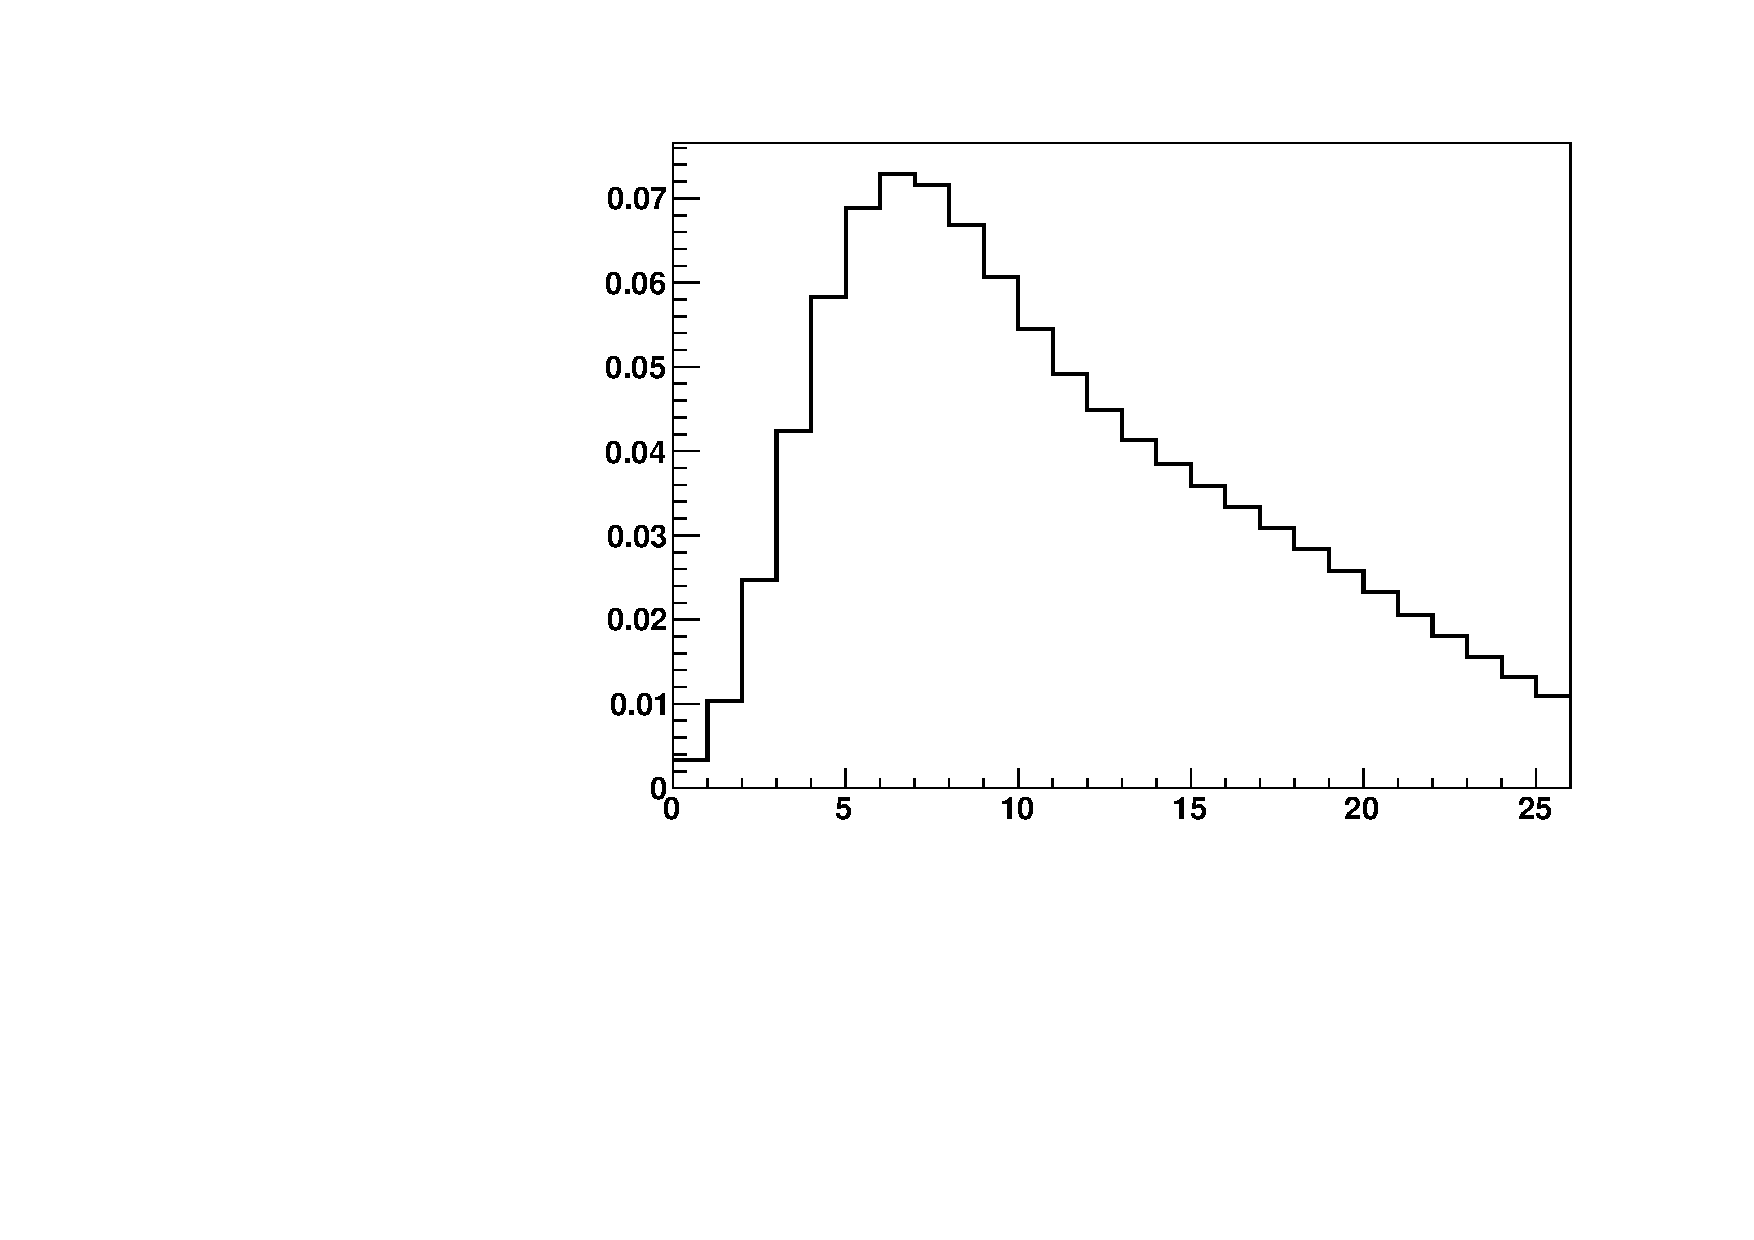
\includegraphics[scale=0.35]{plots/mc_pileup.pdf}
\end{minipage}
\hspace{0.5cm}
\begin{minipage}[b]{0.5\linewidth}
\centering
  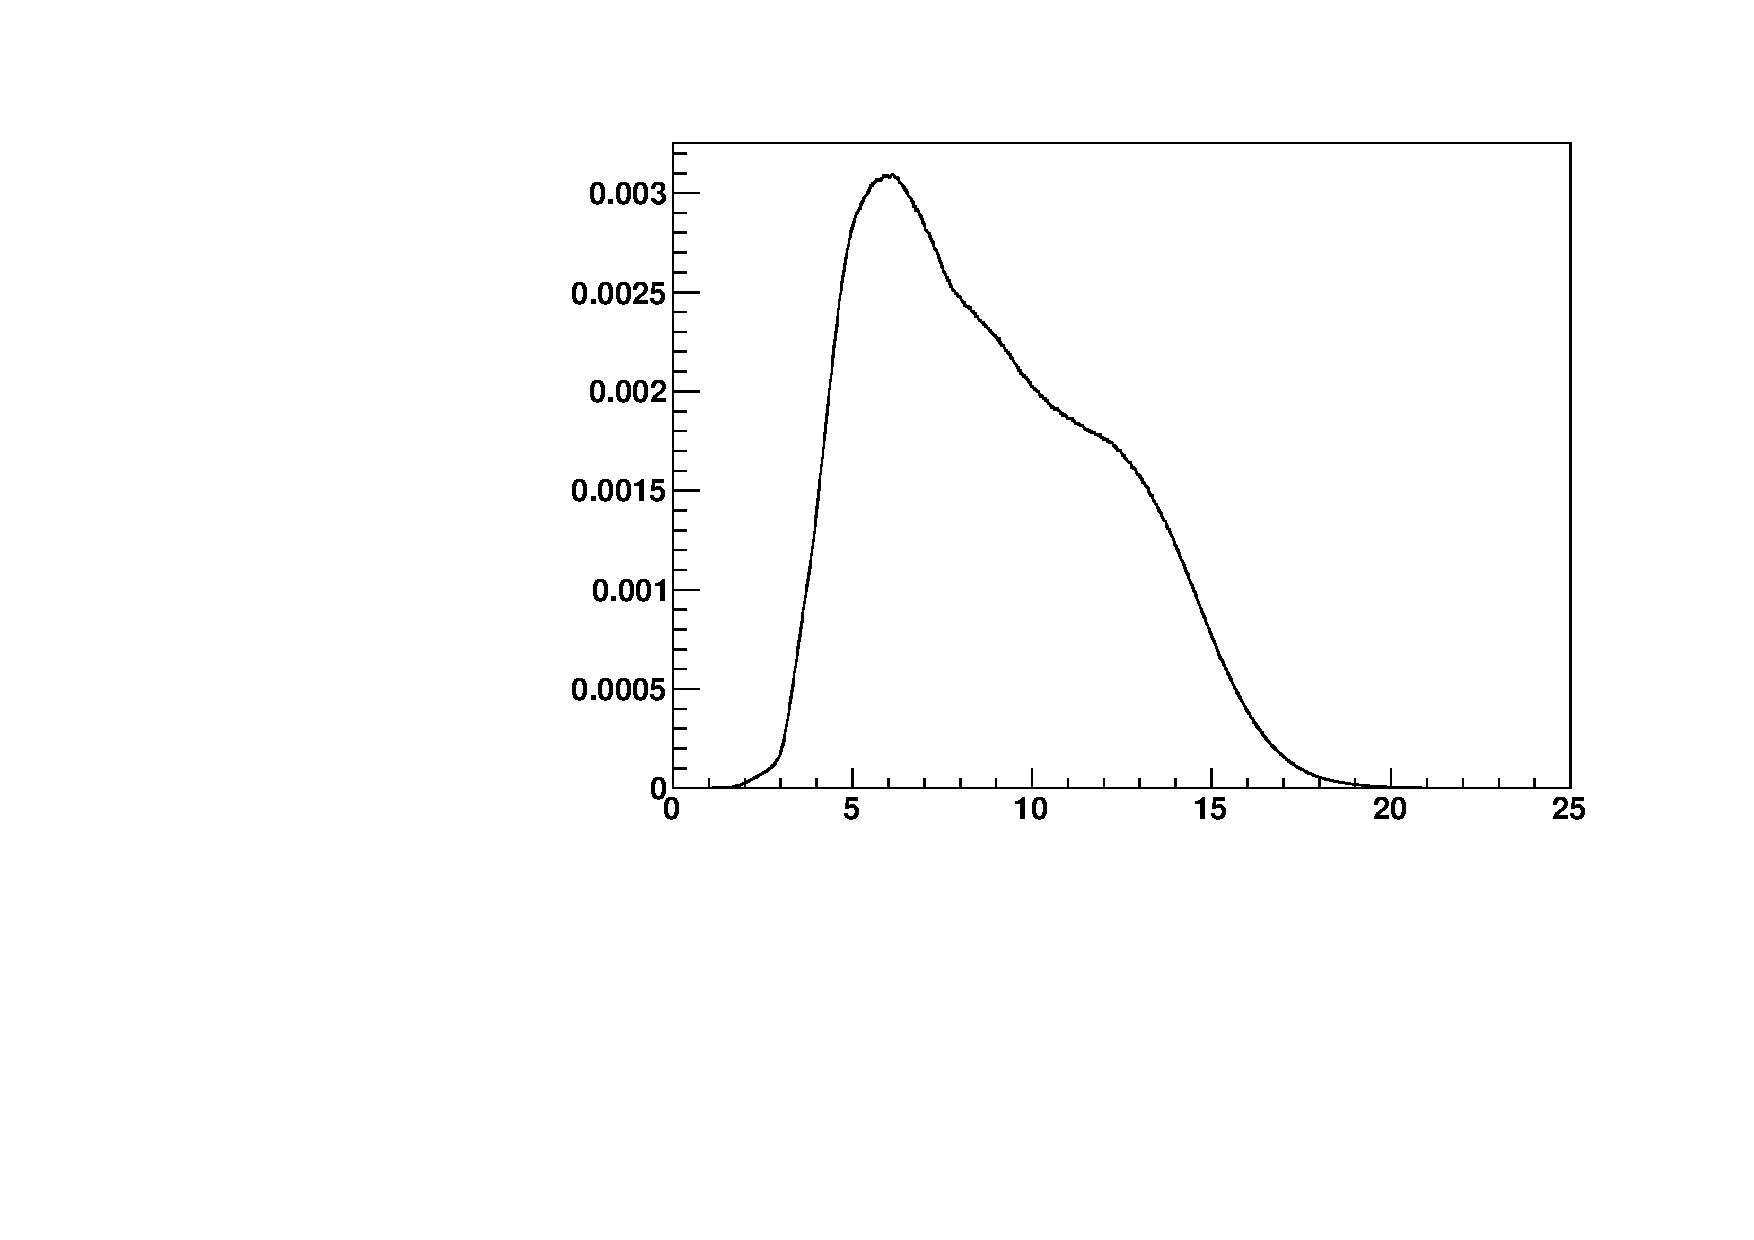
\includegraphics[scale=0.35]{plots/data_pileup.pdf}
\end{minipage}
\caption{Pile-up interaction multiplicity for simulation (left) and the data (right).}
\label{fig:interactionmultiplicity}
\end{figure}
